\documentclass[conference]{IEEEtran}

\IEEEoverridecommandlockouts

\usepackage{cite}
\usepackage{amsmath,amssymb,amsfonts}
\usepackage{algorithmic}
\usepackage{graphicx}
\usepackage{textcomp}
\usepackage{xcolor}
\usepackage{romannum}
\usepackage{stfloats}
\usepackage{balance}



\begin{document}


 
\title{Lectura y procesamiento digital de señales electrocardiográficas\\
\thanks{Agradecemos a la Universidad Tecnológica Nacional por permitirnos
el uso de sus instalaciones y recursos para realizar nuestro proyecto, y a los
docentes de la materia Medidas Electrónicas I: Pablo De Cesare, Franco Zaccra
y Ramiro Germán Rodriguez Colmeiro por su apoyo durante el trabajo}
}

\author{\IEEEauthorblockN{1\textsuperscript{er} Bruno Glecer}
\IEEEauthorblockA{\textit{UTN - FRBA} \\
Buenos Aires, Argentina \\
bglecer@frba.utn.edu.ar
}
\and
\IEEEauthorblockN{2\textsuperscript{do} Jonathan Yujra}
\IEEEauthorblockA{\textit{UTN - FRBA} \\
Buenos Aires, Argentina \\
jonathany@frba.utn.edu.ar
}
}

\maketitle

\begin{abstract}
La técnica de la lectura de señales eléctricas producidas por el corazón se conoce
como electrocardiografía, y es una parte importante de la medicina moderna. En esta
publicación demostramos un circuito básico capaz de captar y digitalizar señales
cardíacas mediante el uso de un par de electrodos colocados sobre un paciente,
conocido como electrocardiografía de única derivación. 
\end{abstract}

\begin{IEEEkeywords}
ECG, bioengineering, filtering, DSP
\end{IEEEkeywords}

\section{Introducción}
 
La técnica de electrocardiografía (ECG) comienza en los fines del siglo \Romannum{19} con
métodos basados en galvanómetros especialmente sensibles y rápidos, con los que se
fue desarrollando los fundamentos de la electrocardiología. Estos métodos fueron
superados por electrocardiógrafos que utilizaban válvulas termoiónicas para la
amplificación de las señales, y estas fueron naturalmente remplazadas por el uso
del transistor. Al día de hoy las señales típicamente son digitalizadas por un
conversor analógico digital (ADC) y procesadas digitalmente para mejorar su claridad. 
En la actualidad, existen métodos que un especialista puede utilizar para analizar
el estado de un corazón a base de las señales obtenidas por un electrocardiógrafo,
esto típicamente se realiza con mediciones tomadas por múltiples electrodos para
lograr una mayor discriminación entre las actividades del ciclo cardíaco.
\cite{ecg_history}

\section{Fundamentos biológicos}

\subsection{Origen de la actividad eléctrica del corazón}

El corazón es un órgano vital presente en la mayoría de los animales que cumple la
función de circular sangre a través de las arterias y venas con el fin de
transportar oxígeno y nutrientes a la gran mayoría de las partes del cuerpo.
El corazón está principalmente compuesto por tejido muscular que se contrae y relaja
en forma coordinada, la secuencia en el que lo realiza se conoce como el
\textit{ciclo cardíaco}. Las contracciones son causadas por señales eléctricas
producidas por el \textit{nódulo sinoauricular}. Debido a que la naturaleza de estas
señales es eléctrica, y debido a que los tejidos húmedos incluyendo la piel tienen
una conductividad eléctrica considerable, es posible realizar mediciones de estas
señales de forma no invasiva mediante la colocación de electrodos en la región
cercana al corazón. Observando las señales es posible identificar las distintas
etapas del ciclo cardíaco, y con suficiente pericia, reconocer la salud del órgano.


Para mayor comprensión, a continuación describiremos las etapas más importantes del
ciclo cardíaco y como se relacionan con una señal electrocardiográfica:
\cite{ecg_workings}

\begin{itemize}
    \item \textbf{Sístole auricular (Onda P)}:
        Durante esta etapa las cavidades superiores llamadas aurículas se contraen
        para enviar la sangre a las respectivas cavidades inferiores llamadas
        ventrículos.
        La aurícula derecha recibe sangre desoxigenada del cuerpo, mientras la
        aurícula izquierda recibe sangre recientemente oxigenada, directo de los
        pulmones.

        Este evento da origen a una señal denominada \textit{onda P}

    \item \textbf{Sístole ventricular (Complejo QRS)}:
        Durante esta etapa los ventrículos se contraen para expulsar la sangre
        al exterior del corazón. El ventrículo derecho envía su sangre desoxigenada
        hacia los pulmones, mientras que el ventrículo izquierdo envía su sangre
        oxigenada al resto del cuerpo.
        Esta etapa es compleja, y su representación eléctrica puede variar, pero
        suele estar compuesta por un pico negativo pequeño denominado \textit{onda Q},
        seguido de un pulso positivo de alta amplitud denominado \textit{onda R} y
        seguido de otro pulso negativo denominado \textit{onda S}. El
        conjunto de estas tres ondas, se las denomina \textit{complejo QRS}.
        
        Dependiendo del estado del corazón, la onda Q y la onda S pueden estar o no
        presentes, mientras que la onda R siempre esta presente y corresponde al
        punto de mayor actividad eléctrica del corazón en todo su ciclo.


    \item \textbf{Diástole Ventricular (Onda T)}:
        En esta etapa los ventrículos se relajan, preparando el corazón para el
        siguiente ciclo. La relajación de los ventrículos se presenta eléctricamente
        como una onda similar a la onda P. A esta onda se la denomina \textit{onda T}.

\end{itemize}

En la figura \ref{fig:ecg_onda} se muestra un diagrama de una señal ECG típica.

\begin{figure}[thb]
    \centerline{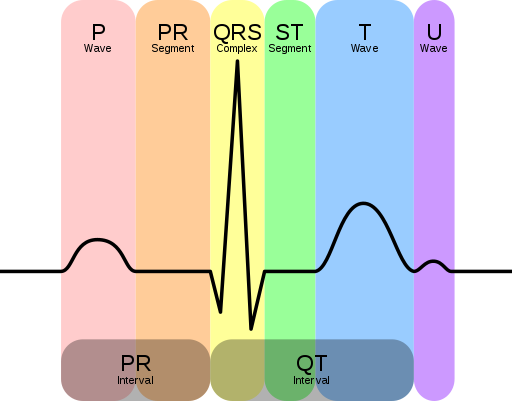
\includegraphics[width=0.9\linewidth]{figs/512px-EKG_Complex_en.svg.png}}
    \caption{Ejemplo de una señal de ECG típica. La última onda "U" no suele ser
    visible debido a su pequeña amplitud, y su naturaleza no está totalmente
    comprendida.}
    \label{fig:ecg_onda}
\end{figure}



\subsection{Características de la señal eléctrica}

Las señales eléctricas captadas por los electrodos tienen amplitudes en el rango de
1-3 mV, dependiendo de la ubicación de los electrodos, su tamaño, características
de la piel del paciente, entre otros factores difíciles de controlar. Además, se
conoce que el rango de frecuencias de interés de la señal es de entre
0.05 Hz y 200 Hz. Por otro lado, la impedancia de salida de la señal puede rondar
los cientos de kiloohmios, lo cual exige una impedancia de entrada alta para el
correcto funcionamiento de un electrocardiógrafo.  
 \cite{ecg_signal_amp} \cite{ecg_signal_freq}


\section{Metodología General}

\subsection{Objetivo de medición}

Nuestra meta para este trabajo fue el diseño y construcción de un electrocardiógrafo
capaz de captar una señal cardíaca con la suficiente calidad para lograr distinguir
la onda P, T y el complejo QRS y de mostrar los valores temporales y de amplitud
lo más precisamente posible.

Por simplicidad, se eligió que su entrada sea de única derivación (un solo par de
electrodos).
\begin{figure*}[b]
    \centering
    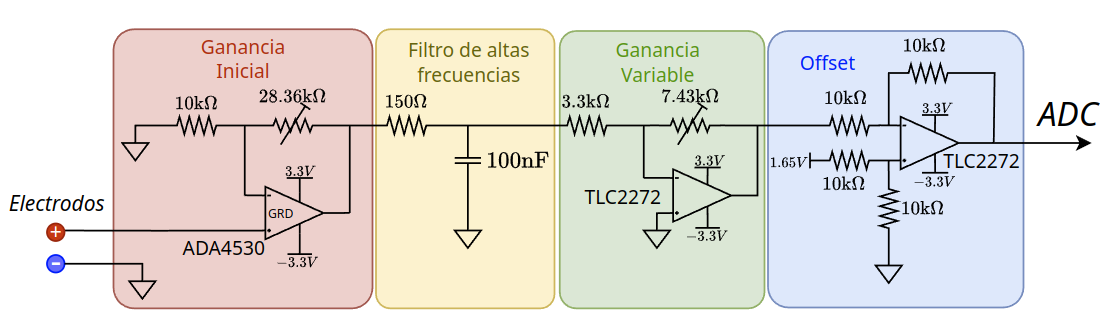
\includegraphics[width=\textwidth]{figs/etapa_analogica.png}
    \caption{Esquemático simplificado de la etapa analógica del módulo desarrollado 
    por el GIBIO en la UTN-FRBA.}
    \label{fig:etapa_analogica_esquematico}
  \end{figure*}
\subsection{Acondicionamiento analógico}




La señal captada por los electrodos debe ser amplificada y filtrada analógicamente
antes de ser digitalizada. La elección de la primera etapa de amplificación es
crítica: es especialmente importante que sea de bajo ruido, debido a la pequeña
señal de entrada, y tiene que operar con mínimo consumo de corriente de polarización
de entrada, debido a la alta impedancia de salida de la señal.

El diseño de esta etapa puede ser complicada y requiere implementarse en un PCB 
con consideraciones de diseño especiales. Para optimizar el proceso, decidimos
reutilizar un módulo para captar señales biológicas diseñado y armado por el grupo
de investigación \textit{GIBIO} en la UTN-FRBA. Este módulo ya tiene diseñada una
etapa de entrada completa que podemos utilizar para este propósito y un ADC
específico para captar señales de ECG, pero desafortunadamente el ADC no se encontraba
funcionando correctamente, entonces nos vimos obligados a utilizar un ADC externo.

El módulo consiste de una etapa de entrada utilizando el amplificador operacional
ADA4530 fabricado por Analog Devices como primera etapa, seguido de una etapa de
filtrado de altas frecuencias, seguido de una etapa de ganancia configurable mediante
el uso de resistencias variables y finalmente una etapa para desplazar la señal hacia
valores positivos y centrarla en 1.65 V, esto es necesario, ya que la referencia
negativa del ADC es de 0 V.

El amplificador operacional ADA4530 \cite{ada4530} es un perfecto candidato para
la primera etapa de amplificación. Tiene una corriente de polarización de entrada de
20 fA. Además, proporciona un terminal de "guard" que permite reducir las perdidas
parásitas de la señal hacia la masa del circuito.
 
La figura \ref{fig:etapa_analogica_esquematico} muestra el esquemático simplificado
del módulo analógico.

Un problema de diseño de este módulo, es que no tiene una frecuencia de corte
superior lo suficientemente baja como para actuar de filtro anti-alias. Esto
puede ser perjudicial para nuestro objetivo y una nueva iteración del circuito
resolvería este error, sin embargo, no se cree que esta falla del diseño cause
mayores complicaciones, debido a que las únicas componentes espectrales por encima
de la frecuencia de Nyquist del ADC y por debajo de la frecuencia de corte del
módulo, consisten de ruido uniformemente distribuido, lo cual en efecto, introducirá
más ruido en la conversión, pero no causará artefactos de alias que puedan
confundirse con la señal ECG.

Dos de las etapas tienen ganancia ajustable mediante el uso de resistencias
variables. Estas resistencias fueron ajustadas y luego medidas, sus valores se
encuentran en la figura \ref{fig:etapa_analogica_esquematico}, estos valores
darán lugar a una ganancia teórica de 8.631 veces. Este valor fue el utilizado para
realizar la calibración más adelante. Su valor exacto no es de gran importancia,
ya que la calibración contempla la compensación por su incertidumbre 


\subsection{Conversión A/D}

Para convertir la señal analógica entregada por el módulo analógico a una señal
digital necesitamos de un ADC capaz de muestrear como mínimo al doble de la
frecuencia máxima presente en una señal ECG (alrededor de 400 muestras por segundo)
para cumplir con el criterio de Nyquist y con una resolución menor a 1 mV para
lograr una buena calidad de la señal.


Se decidió utilizar el ADC ADS1115 de Texas Instruments \cite{ads1115} que adquirimos
ya montando sobre una placa con los componentes auxiliares que necesita el
circuito integrado ya colocados.

Este ADC tiene una frecuencia de muestreo máxima de 860 muestras por segundo, resolución
de 16 bit y una interfaz I$^2$C. Este ADC fue elegido por su gran disponibilidad,
facilidad de uso y también porque cumple con nuestro requisito de ser capaz de
muestrear por arriba de los 400 Hz.

El ADS1115 fue configurado en modo single-shot para utilizar la
base de tiempo del microcontrolador. Estará operando a 500 muestras por
segundo. En términos de resolución, la tensión de referencia positiva fue configurada
para utilizar la referencia interna de 4.096 V, y 0 V como referencia negativa.
Esta configuración permite una resolución teórica de $\dfrac{4.096 V}{2^{16}} = 
62.5 \mu V$.

\subsection{Interfaz PC-ADC}

Para configurar y comunicar los resultados del ADS1115 con una computadora, es
necesario el uso de un microcontrolador. Decidimos utilizar una placa de desarrollo 
de ST Microelectronics: La \textit{Nucleo F401-RE} \cite{nucleo}. Esta placa está
basada sobre un microcontrolador STM32F401RE, este es un ARM Cortex-M4 de 32 bit
con una frecuencia de reloj máxima de 84 MHz. Este microcontrolador está
sobredimensionado para esta aplicación, pero aun así lo utilizamos porque el
grupo ya tenía experiencia previa con esta placa de desarrollo en particular y lo
pudimos obtener con facilidad mediante la universidad.

De este microcontrolador utilizamos principalmente un puerto I$^2$C para la
comunicación con el ADS1115, un timer interno con una interrupción para poder
iniciar una conversión con una frecuencia de 500 Hz y un puerto UART que la placa
de desarrollo utiliza para crear un enlace con la PC mediante el puerto USB.

El programa ejecutándose en el microcontrolador realiza la configuración inicial del
ADS1115, su lectura periódica y la transmisión de los resultados de las conversiones
del ADC mediante un puerto serie.

El código fuente y los binarios utilizados se encuentra en el repositorio del
proyecto. \cite{repository} 

\subsection{Software PC}\label{software-pc}

Para la visualización de la señal, se desarrolló una interfaz gráfica programada
en Python utilizando la librería PyQt5. El programa recibe los datos de las
conversiones del ADC mediante la interfaz del puerto serie establecido a través de
USB con el microcontrolador.

La señal recibida por la PC en este punto del proceso tiene una mala relación señal a
ruido, dificultando mucho su visualización. Para mejorar esto se emplea el uso de
filtros digitales para reducir el ruido, en particular, los ruidos que típicamente
están presentes en la señal son: Interferencias de 50 o 60 Hz causado por la
frecuencia de línea, ruido de baja frecuencia causado por cambios en la conductividad
eléctrica de la piel del paciente y ruido en todo el espectro causado por varias
fuentes de interferencia.

Para mitigar cada una de estas fuentes de ruido, utilizamos dos tipos de filtros
digitales en cascada. Primero, se aplica un filtro notch con frecuencia central de
50 Hz y selectividad de 2. Y segundo, un filtro Butterworth pasabanda de segundo
orden con frecuencias de corte en 0.5 Hz y 100 Hz. Excepto por la frecuencia central
del primer filtro notch, los otros valores fueron elegidos experimentalmente para
mejorar la claridad de la señal. Los valores del filtro pasa banda recortan parte
del espectro de interés de la señal, aun así, la reducción de ruido que acompaña
esta limitación beneficia la claridad de la señal.


\begin{figure}[thb]
    \centerline{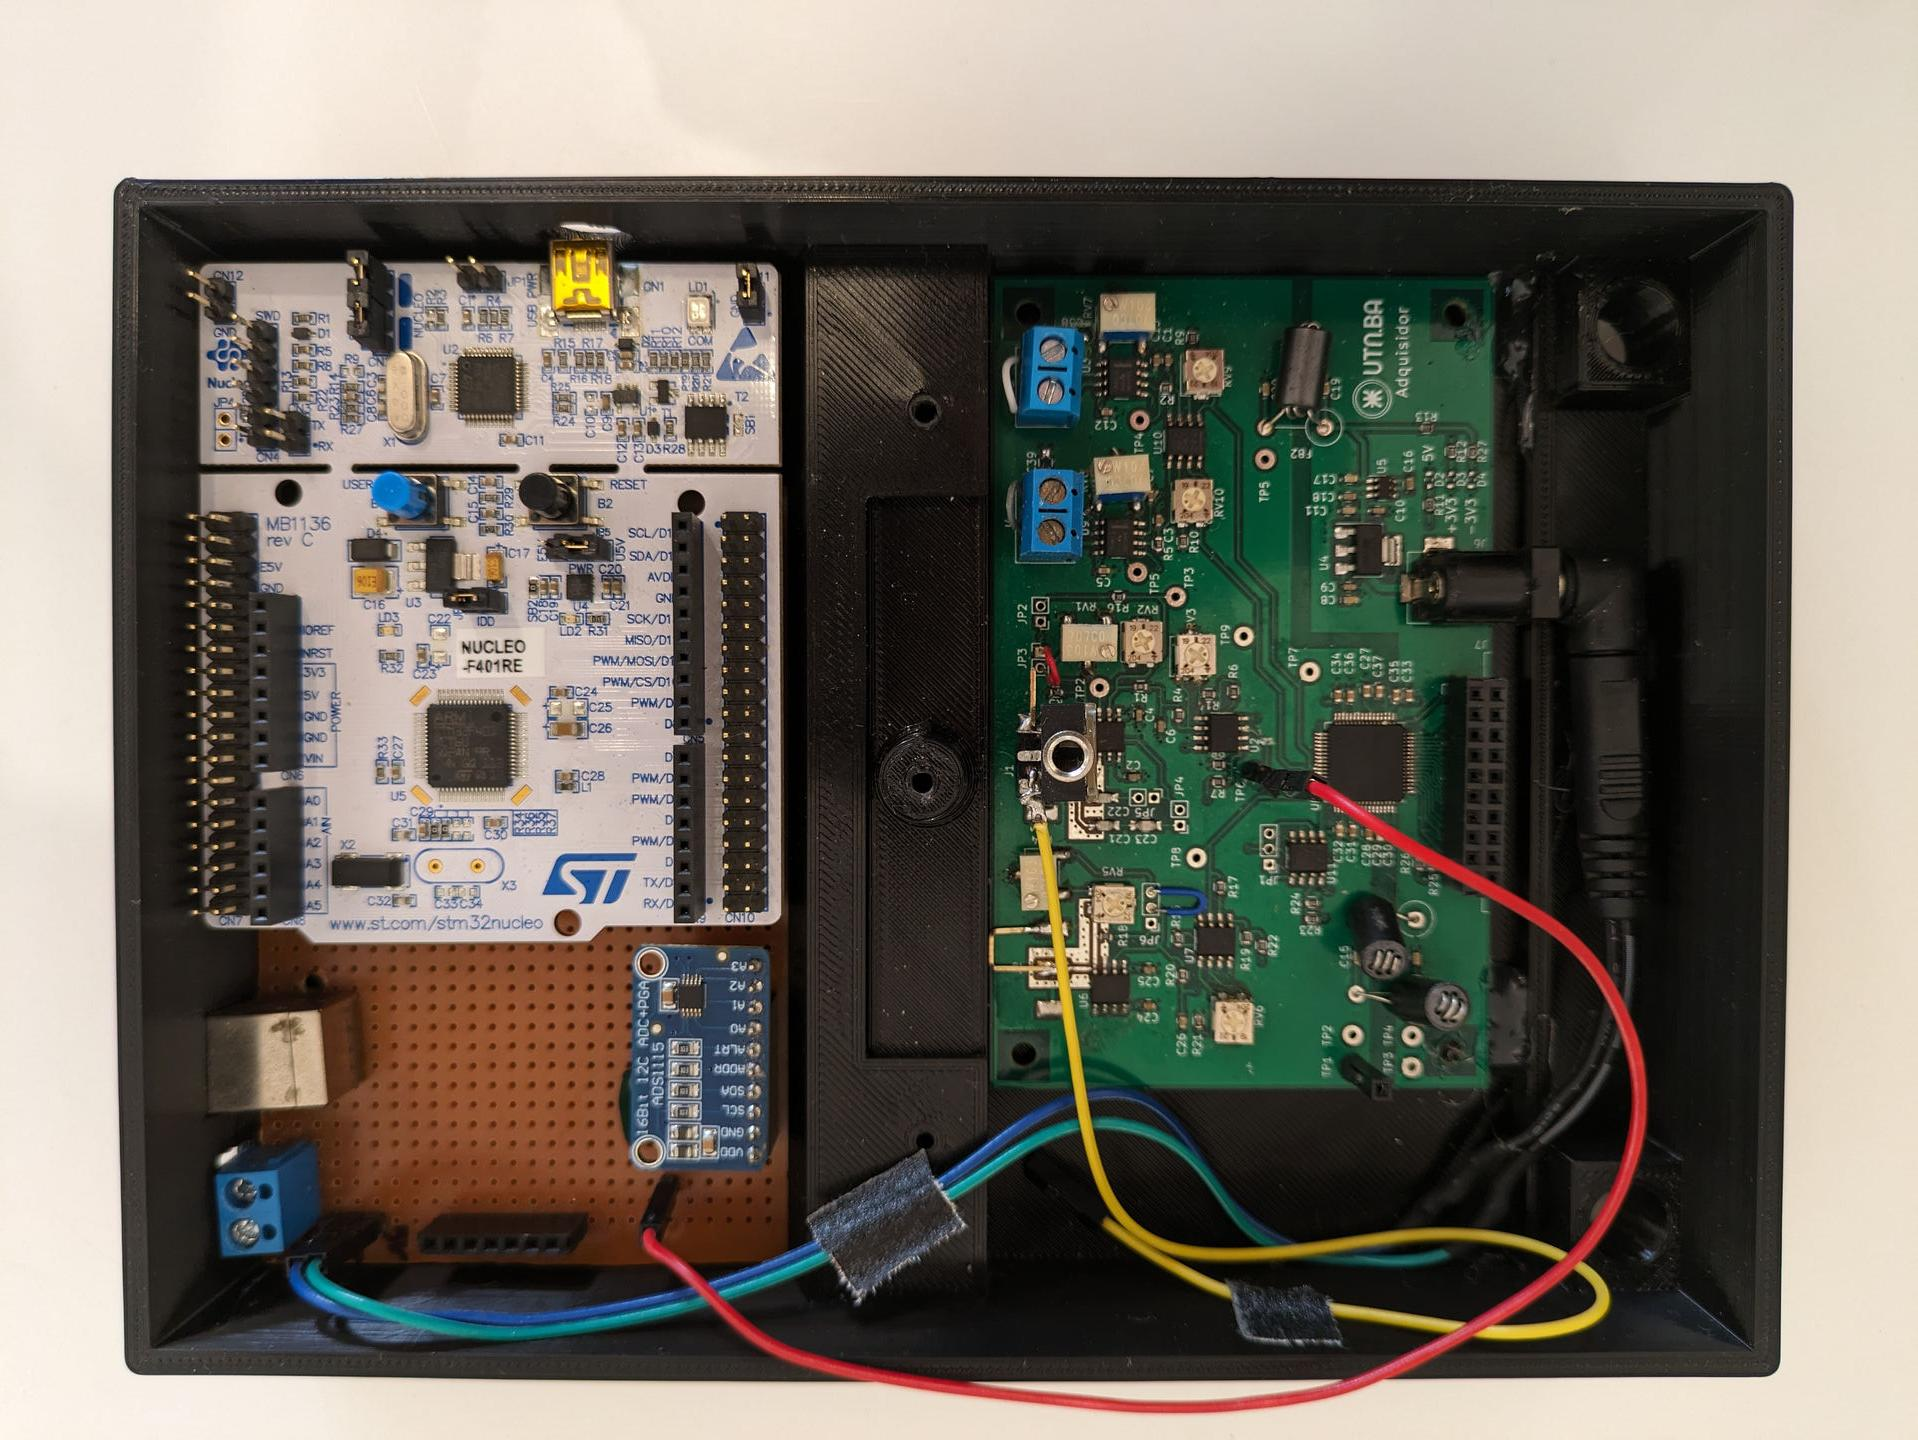
\includegraphics[width=\linewidth]{figs/foto_proyecto.jpeg}}
    \caption{Fotografía del proyecto en su gabinete.}
    \label{fig:foto_proyecto}
    \end{figure}

\section{Calibración}

\subsection{Necesidad}

El electrocardiógrafo desarrollado tiene varias fuentes de incertidumbre, las más
relevantes son la transferencia entre la entrada y la señal digitalizada, y la base
de tiempo utilizada para muestrear la señal. Para que las interpretaciones del
electrocardiograma puedan ser precisas es necesario tener buena linealidad en la 
transferencia y temporizaciones precisas. El objetivo de la calibración es obtener
dos factores: Un factor de corrección temporal que denominaremos $\alpha_T$,
que especifica proporcionalmente cuanto está desviada la base de tiempo del
electrocardiógrafo, y un factor de calibración de amplitud que denominaremos
$\alpha_A$, que especifica la diferencia relativa entre la ganancia teórica del
sistema y la real.

Una vez que se obtienen estos valores, cualquier análisis que se realice sobre
una señal obtenida por el electrocardiógrafo, se puede corregir multiplicando por
el factor de corrección que corresponda al tipo de medición.

Otra necesidad de conocer con exactitud la base de tiempo es para el uso de los
filtros. Estos depende de conocer con precisión la frecuencia de muestreo del ADC.
El rendimiento del filtro notch de 50 Hz es particularmente sensible a una
desviación en la frecuencia de muestreo.


\subsection{Método}


Para evaluar el desempeño del electrocardiógrafo, se utilizó un generador de funciones
Agilent 33522A con su calibración de fábrica como referencia para generar una señal
electrocardiográfica de duración y amplitud conocida.

El instrumento se controló mediante un script en Python que itera por varias
opciones de amplitud y frecuencia cardíaca, cargando la señal al instrumento el cual 
su salida fue conectada directamente a la entrada del electrocardiógrafo. Para cada 
una de estas configuraciones de frecuencia cardíaca y amplitud se tomaron 10
muestras de 10 segundos cada una utilizando el electrocardiógrafo y fueron guardadas
en archivos para luego procesar.

Una vez obtenidas las señales se les aplicó los mismos filtros que el programa de
la visualización utiliza para limpiar la señal.

Las señales proporcionadas al generador de ondas arbitrario fueron sintetizadas 
utilizando la librería de Python \texttt{neurokit2}. \cite{neurokit2}
Esta misma librería se utilizó
luego para analizar las señales captadas por el electrocardiógrafo.

De las señales captadas se midieron dos parámetros para estudiar el rendimiento:

Primero, la frecuencia cardiaca, este valor es un parámetro biológico clave estudiado
en la electrocardiografía, y además proporciona un valor que tiene una correlación
perfectamente lineal con la base de tiempo del electrocardiógrafo, una posible fuente
de error. Fue medido utilizando la función \texttt{ecg\_process} de \texttt{neurokit2}
con  el método de detección de picos "engzeemod2012" y promediando el valor de ritmo
cardíaco a lo largo del vector de salida.

Y como segundo parámetro, se midió la diferencia entra la amplitud promedio de los
pulsos R y la amplitud promedio de los pulsos S. Los pulsos también fueron detectados
utilizando la función \texttt{ecg\_process} con el mismo método de detección de picos
que su usó para obtener la frecuencia cardiaca. Este parámetro es útil, debido a que
representa una buena medición de la amplitud pico a pico de la señal, ya que los
pulsos S son los puntos más bajos de la señal y los pulsos R los más altos.

La calibración se realizó para las frecuencias cardiacas de: 50, 75, 100, 200 y 250
latidos por minuto, y amplitudes de 0.002, 0.005, 0.01, 0.02 y 0.1 V.
Para cada una de estas combinaciones se realizaron 10 muestras de 10 segundos cada
una, resultando en un total de 250 muestras. La mitad de estas muestras fueron
destinadas para la calibración, mientras que la otra  mitad se utilizó para la
verificación de la calibración. Es importante no reutilizar las mismas muestras para
calibrar y para verificar debido a que esto producirá una verificación de la
calibración sesgada.

Una vez que se obtuvieron las mediciones de la calibración, estos se compararon con 
los valores teóricos para calcular ambos factores de corrección.

Más específicamente, cada factor se calculó utilizando la media aritmética
de todos los errores relativos:

$$\alpha_{T} = \dfrac{1}{N} \sum_{(a,f,n) \in A \times F \times \{1...10 \}}\nolimits
~ \frac{f}{\hat{f}_{(a,f,n)}} $$ 
 

$$\alpha_{A} = \dfrac{1}{N} \sum_{(a,f,n) \in A \times F \times \{1...10 \}}\nolimits
~ \frac{a}{\hat{a}_{(a,f,n)}} $$ 
\begin{figure}[b]
    \centering
    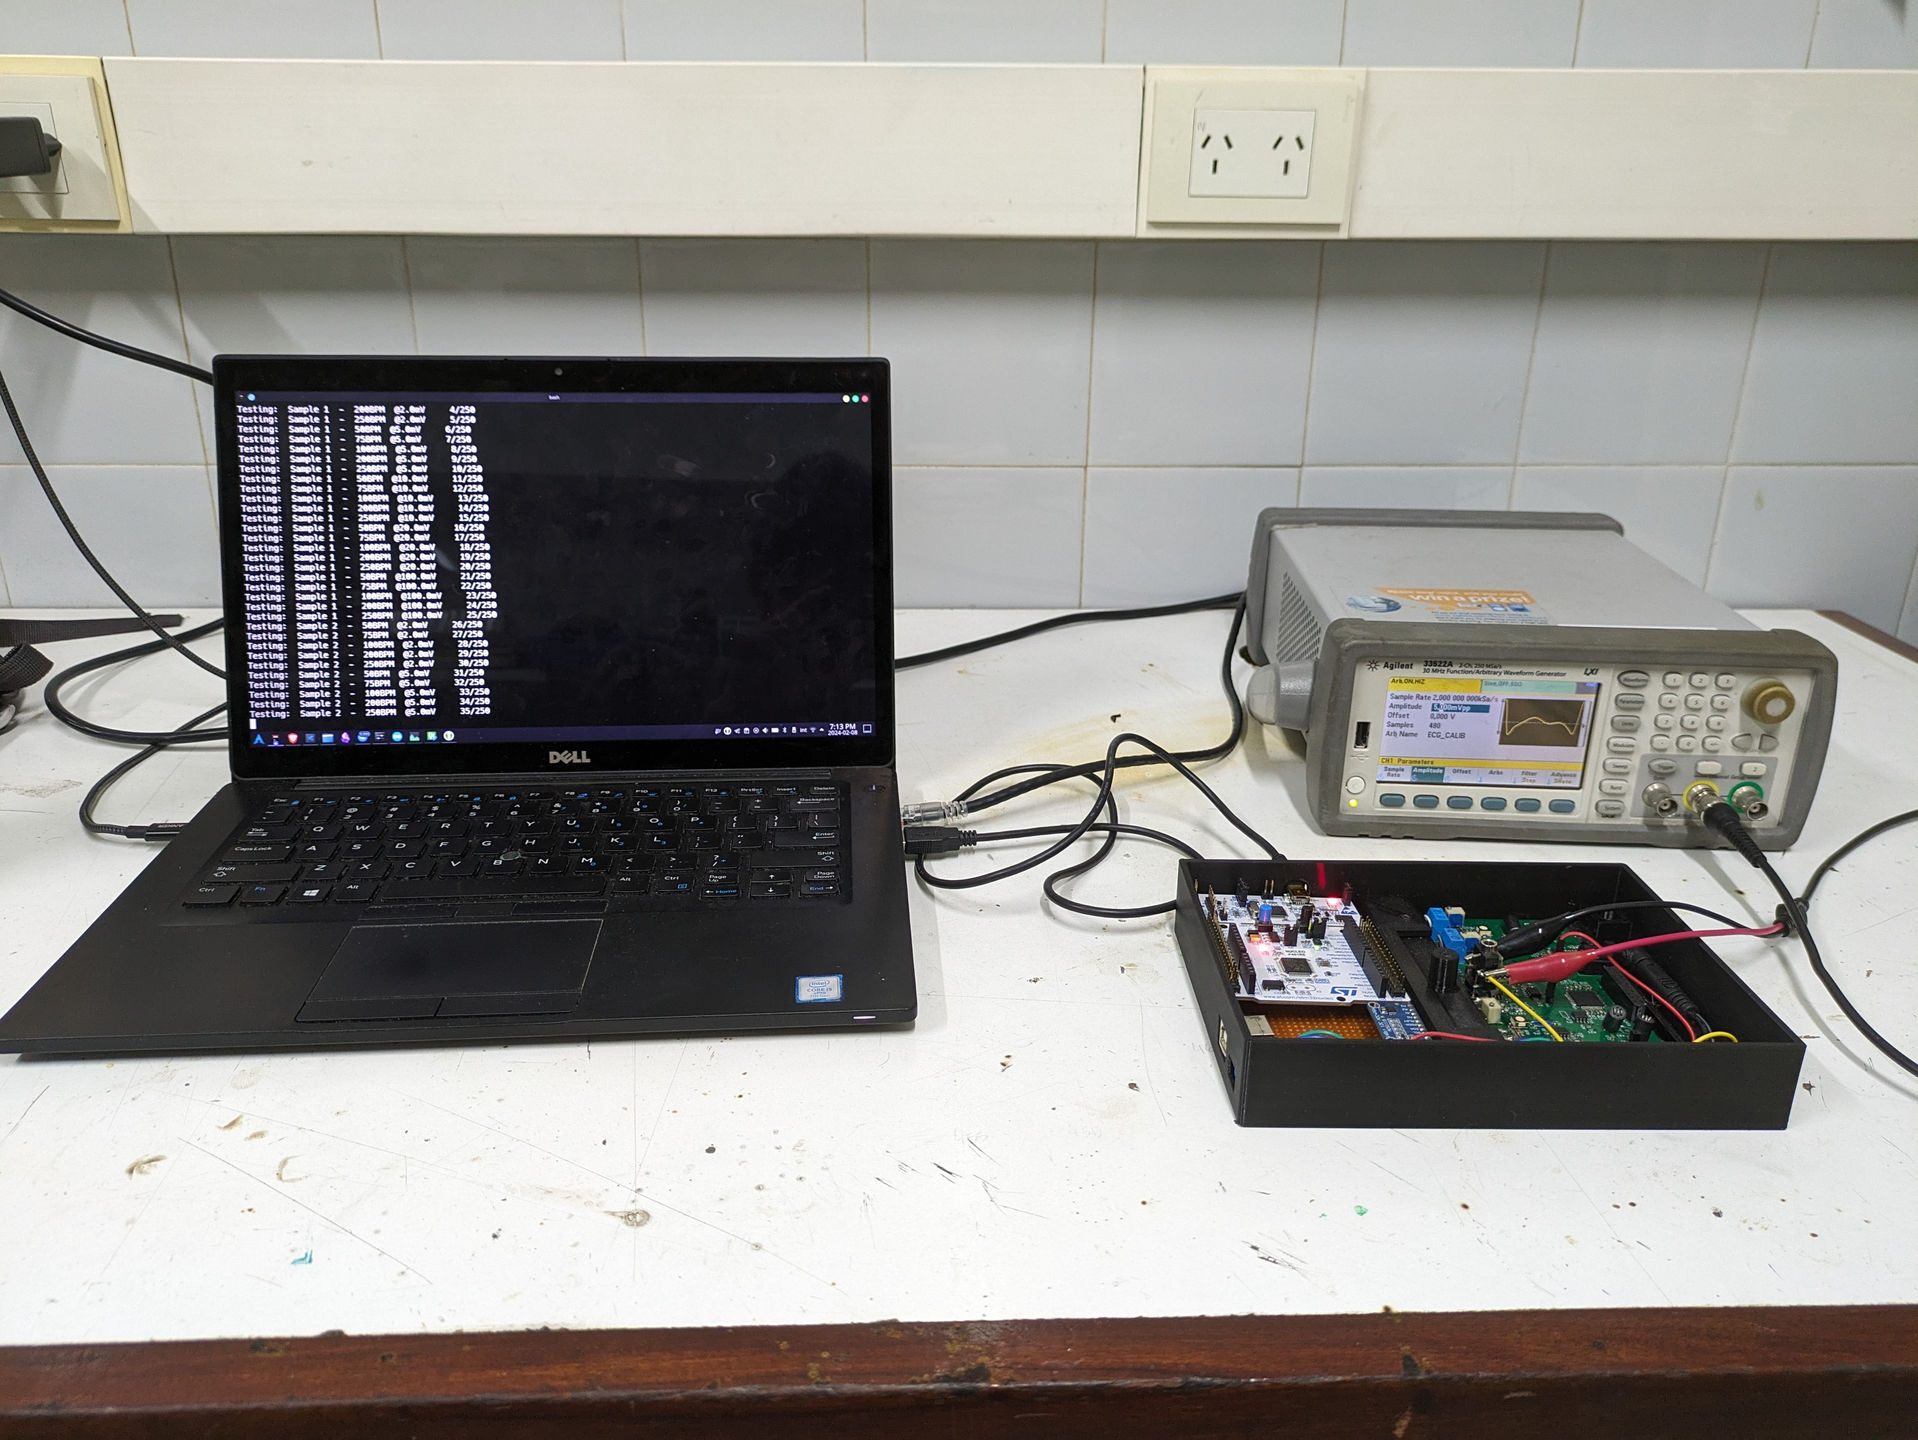
\includegraphics[width=\linewidth]{figs/foto_calibracion.jpeg}
    \caption{Calibración del proyecto en progreso. La medición de las 250 muestras
    demoró aproximadamente una hora.}
    \label{fig:calibracion}

\end{figure}
Donde $A$ y $F$ son respectivamente los conjuntos de amplitudes y frecuencias
cardiacas utilizadas para calibrar. $\hat{f}_{(a,f,n)}$ y $\hat{a}_{(a,f,n)}$ es el valor medido durante
la calibración de la $n$-esima muestra para una amplitud de $a$ y
frecuencia cardíaca de $f$. $N=125$ es la cantidad total de
muestras medidas (5 frecuencias cardiacas, 5 amplitudes y 5 muestras por combinación).

Además, para cada uno de estos factores, es relevante conocer su incertidumbre,
para esto calculamos el desvío estándar de la media de cada uno. Las fórmulas
utilizadas son las siguientes:

$$ u^2 \left( \alpha_{T} \right) = \dfrac{1}{N - 1} \sum_{(a,f,n) \in A \times F
\times \{1...10 \}}\nolimits \left( \frac{f}{\hat{f}_{(a,f,n)}} - \overline{\alpha_{T}}
\right)^2 $$ 

$$ u^2 \left( \alpha_{A} \right) = \dfrac{1}{N - 1} \sum_{(a,f,n) \in A \times F
\times \{1...10 \}}\nolimits \left( \frac{a}{\hat{a}_{(a,f,n)}} - \overline{\alpha_{A}}
\right)^2 $$ 

En todos los casos, la incertidumbre se dará en forma expandida con un factor de
cobertura $k = 2$, es decir, con una confianza del 95\%:

$$U(\alpha) = k u(\alpha)$$

Una vez que se obtienen estos factores de calibración, se pueden utilizar para ajustar
cualquier medición realizada con el electrocardiógrafo utilizando las siguientes
conversiones:

$$ F' = \alpha_{T} F$$

$$ T' = \frac{T}{\alpha_{T}} $$

$$ A' = \alpha_{A} A$$

\begin{figure*}[t]
    \centering
    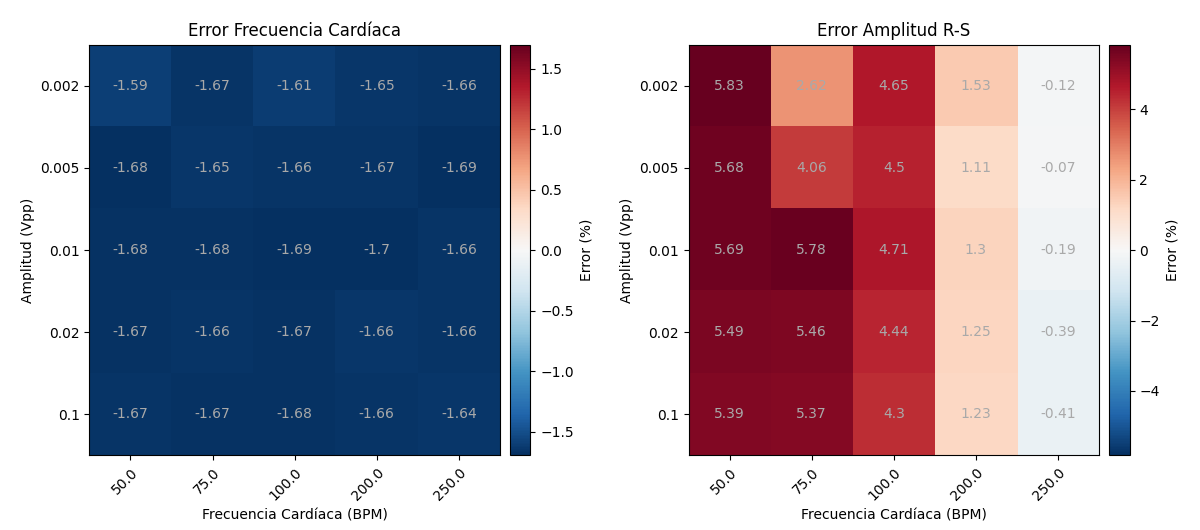
\includegraphics[width=\textwidth]{figs/plot_error_sin_calib.png}
    \caption{Mapa de error de medición sin la calibración aplicada.}
    \label{fig:plot_errpr_sin_calib}

\end{figure*}

Donde $F$ indica algún parámetro frecuencial medido, como ser pulsaciones por minuto,
$T$ indica un parámetro temporal medido como ser separación entre pulsos, y
$A$ indica un parámetro de amplitud.
$F'$, $T'$ y $A'$ indican los valores corregidos de $F$, $T$ y $A$ respectivamente.
 
Otra forma de aplicar una corrección es modificar la señal previo al análisis
de la siguiente forma:

$$ v'(t) = \alpha_{A} ~ v(\alpha_T ~ t)$$

Donde $v(t)$ representa la señal original y $v'(t)$ la señal corregida.

 

\subsection{Resultados de la calibración}

La figura \ref{fig:plot_errpr_sin_calib} muestra para cada frecuencia y amplitud,
el error relativo medio entre la medición de cada parámetro, y el esperado.

 
Analizando cualitativamente el gráfico de error de frecuencia cardíaca, vemos que este
es muy consistente a lo largo de las frecuencias y amplitudes probadas,
todos los valores de error están dentro de un rango del 1.6\% al 1.7\%.

De lo contrario, vemos que el error de amplitud no es consistente y varía
dependiendo de la frecuencia cardíaca.

Utilizando las ecuaciones planteadas en la subsección anterior, procedemos a calcular
los factores de corrección.

\boldmath
$$ \alpha_{T} = 1.01692 \pm 0.00088 $$

$$ \alpha_{A} = 0.969 \pm 0.048 $$
\unboldmath 



\subsection{Rendimiento de la calibración}

Una vez obtenido los factores de corrección, estos valores se pueden utilizar
para refinar el desempeño del electrocardiógrafo calibrado. Procedemos a realizar
el mismo análisis que se realizó para la calibración con el paso adicional de
aplicar los factores de corrección previo al análisis de las señales.

Esto resulta en el mapa de error visualizado en la figura
\ref{fig:plot_errpr_con_calib}.

Los errores de la frecuencia cardíaca se encuentran dentro de un rango del -0.04\% al
0.02\%, mientras que los errores de amplitud tienen más dispersión y, como es de
esperar, siguen manteniendo la correlación entre error y frecuencia cardíaca que 
se observó previo a la calibración. Los valores de este parámetro existen en el 
rango de -3.6\% al 2.9\%.



\begin{figure*}[t]
    \centering
    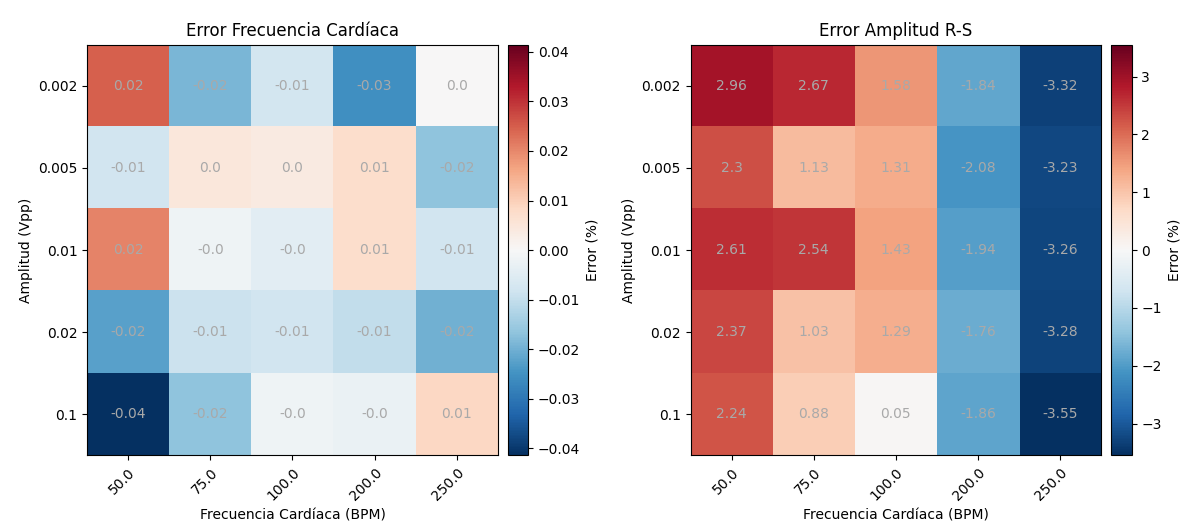
\includegraphics[width=\textwidth]{figs/plot_error_con_calib.png}
    \caption{Mapa de error de medición con la calibración aplicada.}
    \label{fig:plot_errpr_con_calib}

\end{figure*}

\section{Medición de una señal ECG real}


\begin{figure}[t]
    \centering
    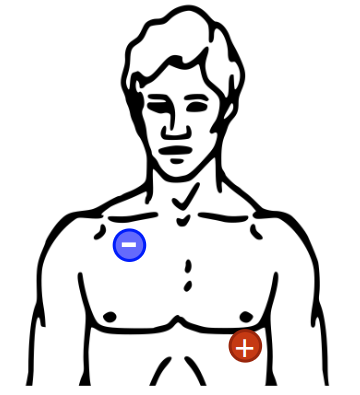
\includegraphics[width=0.5\linewidth]{figs/ubiacion_electrodos.png}
    \caption{Diagrama de la colocación recomendada de los electrodos.}
    \label{fig:ubicacion_electrodos}

\end{figure}
Una vez obtenidos los factores de corrección, estos fueron cargados al programa
que se describió en la sección \ref{software-pc}.

La ubicación de los electrodos es una parte crítica de la electrocardiografía,
basándonos en la literatura y realizando comparaciones cualitativas de la calidad
de la señal obtenida, determinamos que la mejor colocación de los electrodos para
este caso es la ilustrada en la figura \ref{fig:ubicacion_electrodos}

Una vez ubicados los electrodos, y conectados al electrocardiógrafo se puede utilizar
el programa para visualizar la señal obtenida.

En la figura \ref{fig:ecg_real} se muestra una captura de pantalla del graficador
mostrando la señal ECG captada de uno de los integrantes del proyecto.


\begin{figure}[t]
    \centering
    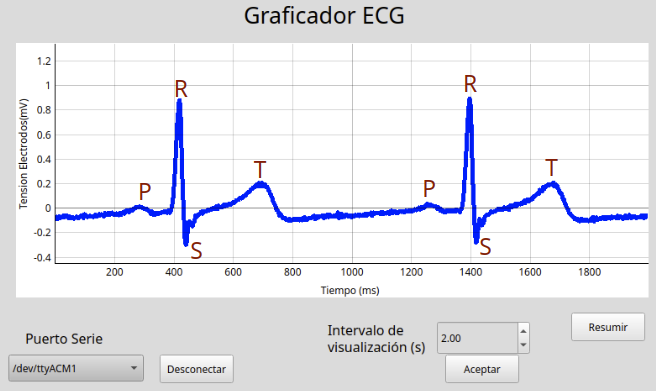
\includegraphics[width=\linewidth]{figs/graficador_ecg_etiquetado.png}
    \caption{Captura de pantalla tomada por la medición del electrocardiógrafo sobre 
    uno de los integrantes del grupo. Se etiquetaron los pulsos claves.}
    \label{fig:ecg_real}

\end{figure}





\section{Conclusiones}

Analizando el error de frecuencia cardíaca previo a la calibración se puede observar
en el mapa de error de la figura \ref{fig:plot_errpr_con_calib} que no varía
dependiendo de frecuencia cardiaca ni de la amplitud.
Esto es un indicador fuerte de que la fuente de esta diferencia es la frecuencia a
la que el ADC se encuentra muestreando. Un estudio del microcontrolador
podría dar más información al respecto. Luego de la calibración, el error de
frecuencia cardiaca permanece debajo del 0.04\%, una cifra muy buena indicando
consistencia entre diferentes condiciones de medición.

En términos de la amplitud, la correlación negativa del valor medido con la
frecuencia cardiaca puede ser un indicio de que la señal alcanza su valor pico
entre dos muestras del ADC. El comportamiento esperado de esta situación es que
disminuya con un incremento de frecuencia, que es precisamente lo que se observa
que sucede.
Para estudiar esto es necesario analizar la forma de onda con más precisión y 
remplazar el ADC por uno que soporte frecuencias de muestreo más altas. La calibración
ayudó a que el error de amplitud se encuentre más uniformemente disperso entre
las distintas frecuencias cardíacas.

Otro valor de interés para observar es la incertidumbre de los factores de corrección.
Como es de esperar, la incertidumbre relativa de $\alpha_T$ es extremadamente bajo,
alrededor de 0.08\%, indicando que las mediciones de tiempo son muy precisas.
En cambio, la incertidumbre relativa de $\alpha_A$ es aproximadamente 11\%.

La prueba de medición de una señal ECG real resultó sorprendentemente exitosa,
la visualización de la señal permite identificar con claridad los pulsos P, R, S y T.
El pulso Q no aparenta estar presente, esto se puede deber a una combinación de
factores, incluyendo la colocación de los electrodos y el estado del paciente,
no necesariamente indica una limitación del electrocardiógrafo. Aun así, no
descartamos la posibilidad de que simplemente se mezcle con el ruido, esto podría
verificarse utilizando un equipo electrocardiográfico profesional.


\bibliographystyle{IEEEtran}

\newpage
\bibliography{references}

\end{document}
 